\documentclass[a4paper,11pt,dvipdfmx]{jsarticle}


% 数式
\usepackage{amsmath,amsfonts}
\usepackage{bm}
\usepackage{physics}
\usepackage{mathtools}
% 画像
\usepackage[dvipdfmx]{graphicx}
\usepackage{circuitikz}
\usepackage{amsmath,amssymb}
\usepackage{siunitx}
\usepackage{float}
\usepackage{tikz}
\usepackage{askmaps}
\usepackage{multirow}
\usepackage{bigstrut}
\usepackage{rotating}
\usepackage{listings}
\usepackage{subcaption}
% 表
\usepackage{makecell}
% その他
\usepackage{url}
\usepackage{ascmac}
\usepackage{cases}
\usepackage{here}
\usepackage{upgreek}
\usepackage{tocloft}  % tocloftパッケージを使う
\usepackage{titlesec} % titlesecパッケージを使う(セクションタイトルのカスタマイズ)

% 画像挿入コマンド
\newcommand{\Figure}[4]{
\begin{figure}[H]
\centering
\includegraphics[width=#1\linewidth]{./images/#2}
\caption{#3}
\label{fig:#4}
\end{figure}
}

\begin{document}

% 日付とかかえてねー
\begin{table}[b]
  \centering
  \begin{tabular}{|c|c|}
    \hline
    報告者     & 22120 222 塚田 勇人 \\
    \hline
    共同実験者 & 22192 234 山本 悠介  \\ & 22060 211 古城 隆人\\
    \hline
    担当者     & 楡井 雅巳 \\
              &  藤澤 義範\\
    &力丸 彩奈\\
    &村田 雅彦\\
    &富岡 雅弘\\
    \hline
    実験年月日 & 2024年12月13日 天気:曇り 気温:22.7℃ 湿度28\verb#%#\\
    & 2024年12月20日 天気:晴れ 気温:19.8℃ 湿度26\verb#%#\\
    & 2025年1月10日 天気:晴れ 気温:23.3℃ 湿度28\verb#%#\\
    & 2025年1月17日 天気:晴れ 気温:23.3℃ 湿度25\verb#%#\\
    & 2025年1月24日 天気:晴れ 気温:21.3℃ 湿度30\verb#%#\\
    \hline
    提出期限   & 2025年2月6日 23:59  \\
    \hline
    提出日     & \today              \\
    \hline
  \end{tabular}
\end{table}

\title{A/D変換回路の設計と製作}
\author{学籍番号:22120 \\ 組番号:222 \\名前:塚田 勇人}
\date{\today}
\maketitle

\newpage

\section{目的}
アナログ信号をデジタル信号に変換するA/D変換回路を設計し,
製作することで,A/D変換の原理を理解する.

\section{原理}
本実験ではA/D変換回路を製作するにあたって,次の回路を設計し,製作する.
\begin{itemize}
  \item 発振回路
  \item カウンタ回路
  \item ラダー回路
  \item ボルテージフォロア回路
  \item 比較回路
  \item 遅延回路
  \item ラッチ回路
  \item デコーダ回路
\end{itemize}
それぞれについて説明する.

\subsection{発振回路}
発振回路は,周波数を発生させる回路である.無安定マルチバイブレータ
を用いて発振回路を設計する.
%無安定マルチバイブレータの原理を示す。
無安定マルチバイブレータは2つのトランジスタを交互にオン,オフさせることで周波数を発生させる.
外部からのトリガなしに自己発振することができる.\cite{densi}

使用した部品を\ref{tab:oscillationparts}に示す.
\begin{table}[H]
  \centering
  \caption{発振回路に使用した部品}
  \begin{tabular}{|c|c|c|c|}
    \hline
    部品名 & 型番 & 数量  \\
    \hline
    コンデンサ & 積層セラミックコンデンサ1[nF] & 2  \\
    抵抗器 & 炭素被膜抵抗300[$\Omega$]誤差$\pm$5\% & 2 \\
    抵抗器 & 炭素被膜抵抗10[k$\Omega$]誤差$\pm$5\% & 2 \\
    トランジスタ & 2SC1815 & 2  \\
    ピンヘッダ & 2 $\times$ 7 0.1[inch]ピッチ & 1  \\
    \hline
  \end{tabular}
  \label{tab:oscillationparts}
\end{table}

発振器には様々な種類がある.発振器の種類とその特徴についてまとめた表を表\ref{tab:oscillation}に示す.\cite{densi}

\begin{table}[H]
  \centering
  \caption{発振器の種類と特徴}
  \begin{tabular}{|c|c|c|}
    \hline
    発振器の種類 & 特徴  \\
    \hline
    RC発振器 & 抵抗,コンデンサ,オペアンプから構成される.安定性がたかくないが,低周波数帯で使用される.  \\
    LC発振器 & コイル,コンデンサ,トランジスタから構成される.安定しており,高周波数帯で使用される.  \\
    水晶発振器 & 安定性が非常に高く,時計などに使用される.  \\
    \hline
  \end{tabular}
  \label{tab:oscillation}
\end{table}




\subsection{カウンタ回路}
カウンタ回路は,カウントを行う回路である.今回は,汎用ロジックICの一種である
74LS161を用いて設計する.
これはMOS FET(Metal Oxide Semiconductor Field Effect Transistor)となっており,
発振回路から出力された電圧を入力として受け取り,カウントを行う.
また,信号のレベルはCMOS(Complementary Metal Oxide Semiconductor)となっている.
他のレベルとしてTTLレベルがある.
二つのレベルの違いを表\ref{tab:level}に示す。\cite{digital}

\begin{table}[H]
  \centering
  \caption{信号レベルの違い}
  \begin{tabular}{|c|c|c|}
    \hline
    レベル & 特徴  \\
    \hline
    CMOS & 電圧駆動,消費電力が小さい,動作が不安定,体積が小さい  \\
    TTL & 電流駆動,駆動能力が高い  \\
    \hline
  \end{tabular}
  \label{tab:level}
\end{table}

使用した部品を\ref{tab:counterparts}に示す。
\begin{table}[H]
  \centering
  \caption{カウンタ回路に使用した部品}
  \begin{tabular}{|c|c|c|c|}
    \hline
    部品名 & 型番 & 数量  \\
    \hline
    IC & 74LS161 & 1  \\
    ICソケット & 16ピン & 1  \\
    コンデンサ & 積層セラミックコンデンサ0.1[\rm{$\mu$}F] & 1  \\
    \hline
  \end{tabular}
  \label{tab:counterparts}
\end{table}


\subsection{ラダー回路}

ラダー回路は,デジタル信号をアナログ信号に変換する回路である.
ラダー回路は,図\ref{fig:ladder}のように構成されている.

\Figure{0.5}{ladder.png}{ラダー回路}{ladder}

%ディジタル値が1,2の時のアナログ値の出力の計算方法を示す.
もしこの回路に$1 = (001)_2$の値を入力すると以下のような計算が行われる.
まず合成抵抗$R_c$を求める.
\texttt{R4},\texttt{R5}が直列に接続されていて,それに対し,\texttt{R6}が並列に接続されている.またそれに対し,\texttt{R7}が直列に接続されている.
したがって,式\eqref{eq:rc}のように合成抵抗$R_c$を求めることができる.
\begin{equation}
  R_c = R4 + R5 + \frac{R6 \times R7}{R6 + R7} = 10 + 10 + \frac{20 \times 20}{20 + 20} = 40[\rm{k\Omega}]
  \label{eq:rc}
\end{equation}

次に電圧$V_{\text{out}}$を求める.
VCCは5[V]であるため,$V_{\text{out}}$は式\eqref{eq:vout}のように求めることができる.

\begin{equation}
  V_{\text{out}} = \frac{R5}{R3 + R5} \times VCC \times \frac{R4}{R4 + R5} =\frac{10kΩ}{30kΩ} \times 5V \times \frac{10kΩ}{20kΩ} = 1.67V \times 0.5 = 0.625V
  \label{eq:vout}
\end{equation}
このようにして,ディジタル値が1の時のアナログ値が0.625[V]であることがわかる.

同じようにディジタル値が2の時のアナログ値も求めることができる.R5とR6が並列に接続されており,それに対しR4が直列に接続されている.
また,それに対しR2が並列に接続されている.
したがって,次のように合成抵抗$R_c$を求めることができる.

\begin{equation}
  R_456 = \frac{R5 \times R6}{R5 + R6} + R4 = \frac{10 \times 20}{10 + 20} + 10 = 16.67[\rm{k\Omega}]
\end{equation}

\begin{equation}
  R_c = \frac{R2 \times R_456}{R2 + R_456} = \frac{20 \times 16.67}{20 + 16.67} = 9.09[\rm{k\Omega}]
\end{equation}

次に電圧$V_{\text{out}}$を求める.

\begin{equation}
  V_{\text{out}} = VCC \times \frac{R_456}{R2 + R_456} \times \frac{R5}{R4 + R5} = 5 \times \frac{16.67}{36.67} \times \frac{10}{20} = 2.5[V] \times 0.5 = 1.25[V]
\end{equation}

このようにして,ディジタル値が2の時のアナログ値が1.25[V]であることがわかる.

\begin{table}[H]
  \centering
  \caption{ラダー回路に使用した部品}
  \begin{tabular}{|c|c|c|c|}
    \hline
    部品名 & 型番 & 数量  \\
    \hline
    抵抗器 & 金属被膜抵抗10[k$\Omega$]誤差$\pm$1\% & 2  \\
    抵抗器 & 金属被膜抵抗20[k$\Omega$]誤差$\pm$1\% & 4  \\
    \hline
  \end{tabular}
  \label{tab:ladderparts}
\end{table}

\subsection{ボルテージフォロア回路}
ボルテージフォロア回路は,インピーダンスを下げるために使用する回路である.
使用した部品を\ref{tab:voltagefollowerparts}に示す。

\begin{table}[H]
  \centering
  \caption{ボルテージフォロア回路に使用した部品}
  \begin{tabular}{|c|c|c|c|}
    \hline
    部品名 & 型番 & 数量  \\
    \hline
    IC & LMC6482AIN & 1  \\
    コンデンサ & 積層セラミックコンデンサ0.1[\rm{$\mu$}F] & 1  \\
    \hline
  \end{tabular}
  \label{tab:voltagefollowerparts}
\end{table}

\subsection{比較回路}
比較回路は,ラダー回路で変換された信号とアナログ信号生成基板で生成された信号を比較する回路である.
使用した部品を\ref{tab:comparatorparts}に示す。
今回の比較回路の出力はオープンコレクタ出力となっている.
オープンコレクタ出力とは,コレクタが空いている,と訳すように,コレクタが外部に接続されていない状態を指す.
この時にトランジスタがONの時にコレクタがGNDに接続されLowが出力され,OFFの時にはHighが出力される,という動作原理にしたいため,
オープンコレクタにはプルアップ抵抗が接続される.

\begin{table}[H]
  \centering
  \caption{比較回路に使用した部品}
  \begin{tabular}{|c|c|c|c|}
    \hline
    部品名 & 型番 & 数量  \\
    \hline
    IC & LM339 & 1  \\
    コンデンサ & 積層セラミックコンデンサ0.1[\rm{$\mu$}F] & 1  \\
    抵抗 & 炭素被膜抵抗10[k$\Omega$]誤差$\pm$5\% & 2  \\
    \hline
  \end{tabular}
  \label{tab:comparatorparts}
\end{table}

\subsection{遅延回路}
遅延回路は,比較回路で生成された信号を遅延させる回路である.
信号の発生と表示を同時に行ってしまうと,回路の動作が不安定になるため,タイミングをずらすために使用する.
使用した部品を\ref{tab:delayparts}に示す。

\begin{table}[H]
  \centering
  \caption{遅延回路に使用した部品}
  \begin{tabular}{|c|c|c|c|}
    \hline
    部品名 & 型番 & 数量  \\
    \hline
    IC & 74LS0175 & 1  \\
    コンデンサ & 積層セラミックコンデンサ0.1[\rm{$\mu$}F] & 1  \\
    \hline
  \end{tabular}
  \label{tab:delayparts}
\end{table}

\subsection{ラッチ回路}
ラッチ回路は,遅延回路で遅延させた信号を保持する回路である.
使用した部品を\ref{tab:latchparts}に示す。

\begin{table}[H]
  \centering
  \caption{ラッチ回路に使用した部品}
  \begin{tabular}{|c|c|c|c|}
    \hline
    部品名 & 型番 & 数量  \\
    \hline
    IC & 74LS175 & 2  \\
    コンデンサ & 積層セラミックコンデンサ0.1[$\mu$F] & 2  \\
    \hline
  \end{tabular}
  \label{tab:latchparts}
\end{table}

\subsection{デコーダ回路}
デコーダ回路は,入力された信号に対応するディジタル値を表示する回路である.

\section{実験方法}
今回の課題に用いた機器や電子部品について表\ref{tab:equipment}と表\ref{tab:electronicParts}に示す.

\begin{table}[H]
  \caption{実験に用いた機器}
  \centering
  \begin{tabular}{|c|c|c|}
    \hline
    器具名           & 製造元         & 計器番号        \\
    \hline
    はんだごて       & HOZAN          & H-600           \\
    \hline
    オシロスコープ   & テクトロニクス & MSO2014B        \\
    \hline
    ブレッドボード   & SanHayato      & SRH32           \\
    \hline
    ユニバーサル基板 &                & PIC0 94V-O 2344 \\
    \hline
  \end{tabular}
  \label{tab:equipment}
\end{table}

\begin{table}[H]
  \caption{実験に用いた電子部品}
  \centering
  \begin{tabular}{|c|c|c|c|}
    \hline
    部品名                   & 諸元         & 個数 & 部品記号       \\
    \hline
    炭素被膜抵抗             & 300[$\Omega$ ] & 2    & R1~R2         \\
    \hline
    炭素被膜抵抗             & 10[k$\Omega$ ] & 2    & R3~R4,R9~R10 \\
    \hline
    金属皮膜抵抗             & 10[k$\Omega$ ] & 2    & R8~R9         \\
    \hline
    金属皮膜抵抗             & 20[k$\Omega$ ] & 2    & R5~R7,R10     \\
    \hline
    トランジスタ             & 2SC1815      & 2    & T1~T2         \\
    \hline
    積層セラミックコンデンサ & 1[nF]        & 2    & C1~C2         \\
    \hline
    積層セラミックコンデンサ & 0.1[$\mu$F]   & 5    & C3~C7         \\
    \hline
    ICソケット               & 16ピン       & 1    & -              \\
    \hline
    集積回路(IC)1            & 74HC161      & 1    & IC1            \\
    \hline
    集積回路(IC)2            & LMCC6482AIN  & 1    & IC2            \\
    \hline
    集積回路(IC)3            & LM339        & 1    & IC3            \\
    \hline
    集積回路(IC)4            & 74LS175      & 3    & IC4~IC6       \\
    \hline
  \end{tabular}
  \label{tab:electronicParts}
\end{table}

本実験で,初めて作成した回路について動作確認を行う.

\subsection{発振回路}
発振回路の動作確認を行う.ここでは,発振回路のCLKと$\overline{\text{CLK}}$の信号をオシロスコープで観測し,タイミングチャートが図\ref{fig:clock}のようになることを確認する.
図から,周期が14[us]であることがわかるため,逆数をとり,周波数を求めると,71.4[kHz]となる.

\begin{figure}[H]
  \centering
  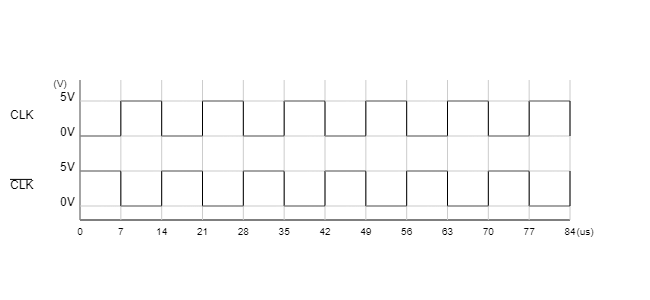
\includegraphics[width=0.8\linewidth]{./images/clock.png}
  \caption{発振回路のタイミングチャート}
  \label{fig:clock}
\end{figure}

\subsection{カウンタ回路}
カウンタ回路の動作確認を行う.
ここでは,カウンタ回路の$\text{D}_0$から$\text{D}_2$をオシロスコープで観測し,CLKとの関係を示すタイミングチャートが図\ref{fig:counter}のようになることを確認する.

\begin{figure}[H]
  \centering
  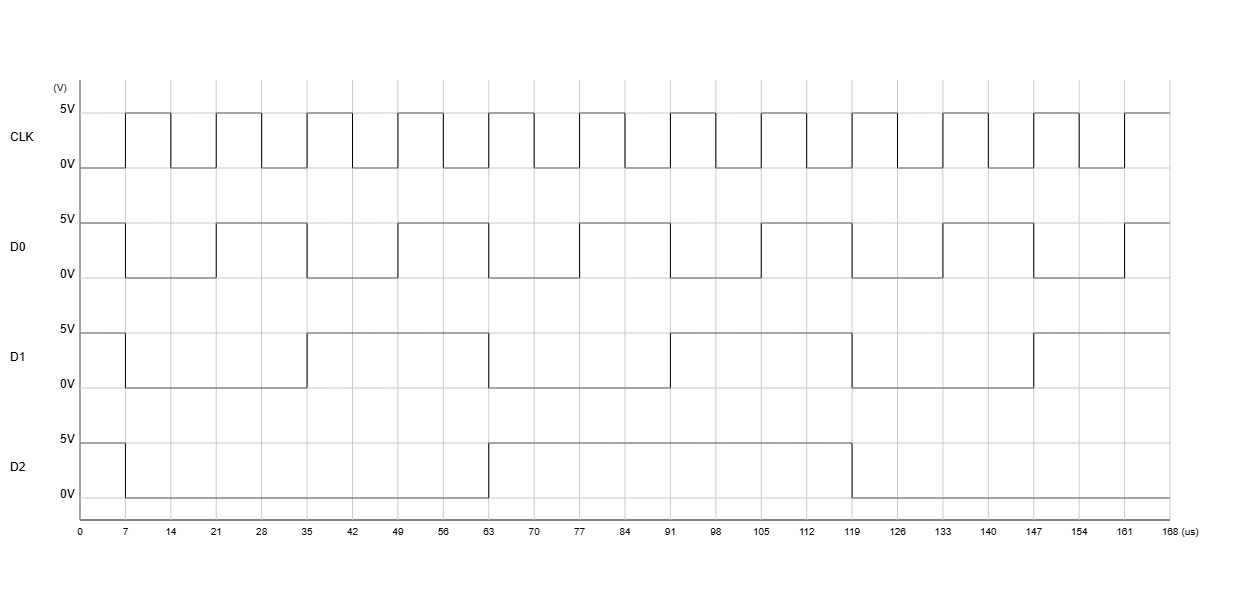
\includegraphics[width=0.8\linewidth]{./images/count.png}
  \caption{カウンタ回路のタイミングチャート}
  \label{fig:counter}
\end{figure}

\subsection{ラダー回路}
ラダー回路の動作確認を行う.
TP5に接続された信号をオシロスコープで観測し,図\ref{fig:ladder}のようなアナログ信号の波形が表示されることを確認する.

\begin{figure}[H]
  \centering
  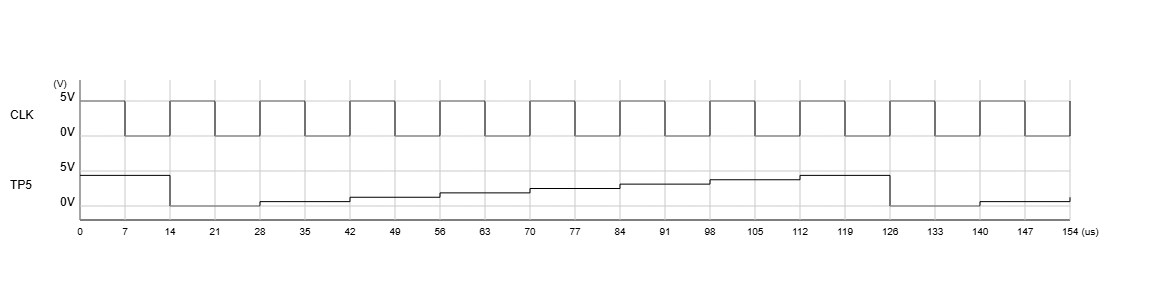
\includegraphics[width=0.8\linewidth]{./images/TP5.png}
  \caption{ラダー回路の波形}
  \label{fig:ladder}
\end{figure}

\subsection{ボルテージフォロア回路}
ボルテージフォロア回路の動作確認を行う.
TP6とAREFで同じ電圧が出ていることを,オシロスコープで観測し,図\ref{fig:voltagefollower}のような波形が表示されることを確認する.

\begin{figure}[H]
  \centering
  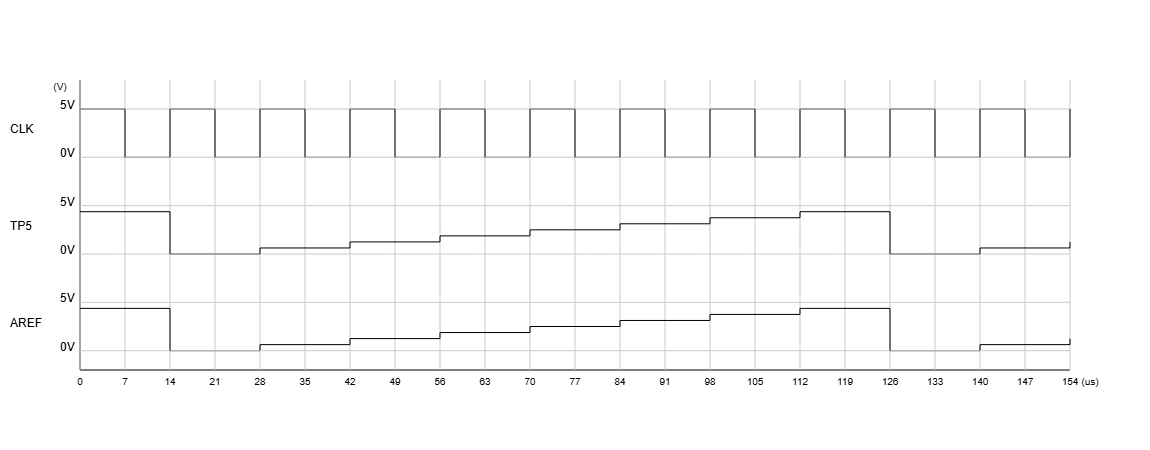
\includegraphics[width=0.8\linewidth]{./images/AREF.png}
  \caption{ボルテージフォロア回路の波形}
  \label{fig:voltagefollower}
\end{figure}

\subsection{比較回路}
比較回路の動作確認を行う.
アナログ信号生成基板の可変抵抗器を操作し,$AIN_0$を2[V]に設定する.
この時のTP6とTP8の波形をオシロスコープで観測し,図\ref{fig:comparator}のような波形が表示されることを確認する.

\begin{figure}[H]
  \centering
  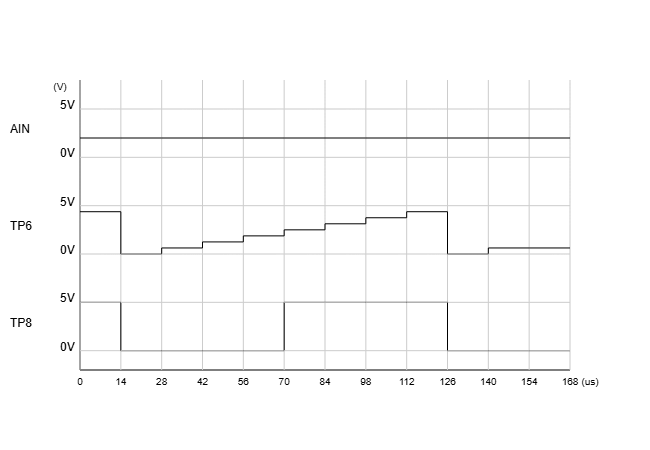
\includegraphics[width=0.8\linewidth]{./images/2V.png}
  \caption{比較回路の波形}
  \label{fig:comparator}
\end{figure}

また,$AIN_0$を3[V]に設定し,TP6とTP8の波形をオシロスコープで観測し,図\ref{fig:comparator2}のような波形が表示されることを確認する.

\begin{figure}[H]
  \centering
  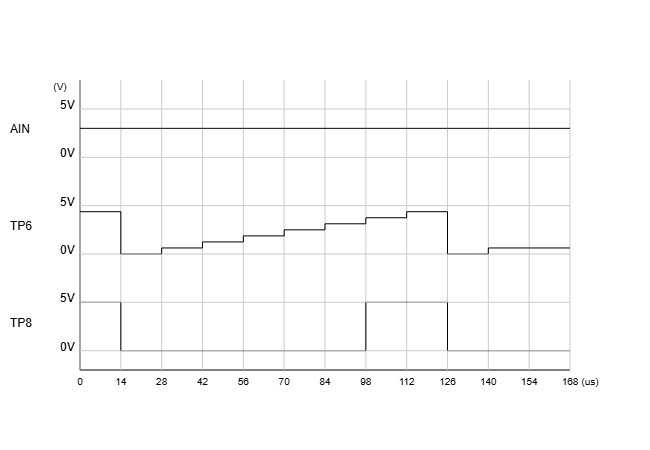
\includegraphics[width=0.8\linewidth]{./images/3V.png}
  \caption{比較回路の波形}
  \label{fig:comparator2}
\end{figure}

最後に,$AIN_0$を0[V]から5[V]まで変化させ,TP8が変化する時の電圧の値が,0.04[V],0.68[V],1.20[V],1.80[V],2.40[V],3.00[V],3.50[V]で
あることを確認する.

\subsection{遅延回路}
遅延回路の動作確認を行う.
$D_0$から$D_2$の信号が,$DP_0$から$DP_2$とCLKの周期の半分遅れていることをオシロスコープで観測し,図\ref{fig:delay}のような波形が表示されることを確認する.

\begin{figure}[H]zikj
  \centering
  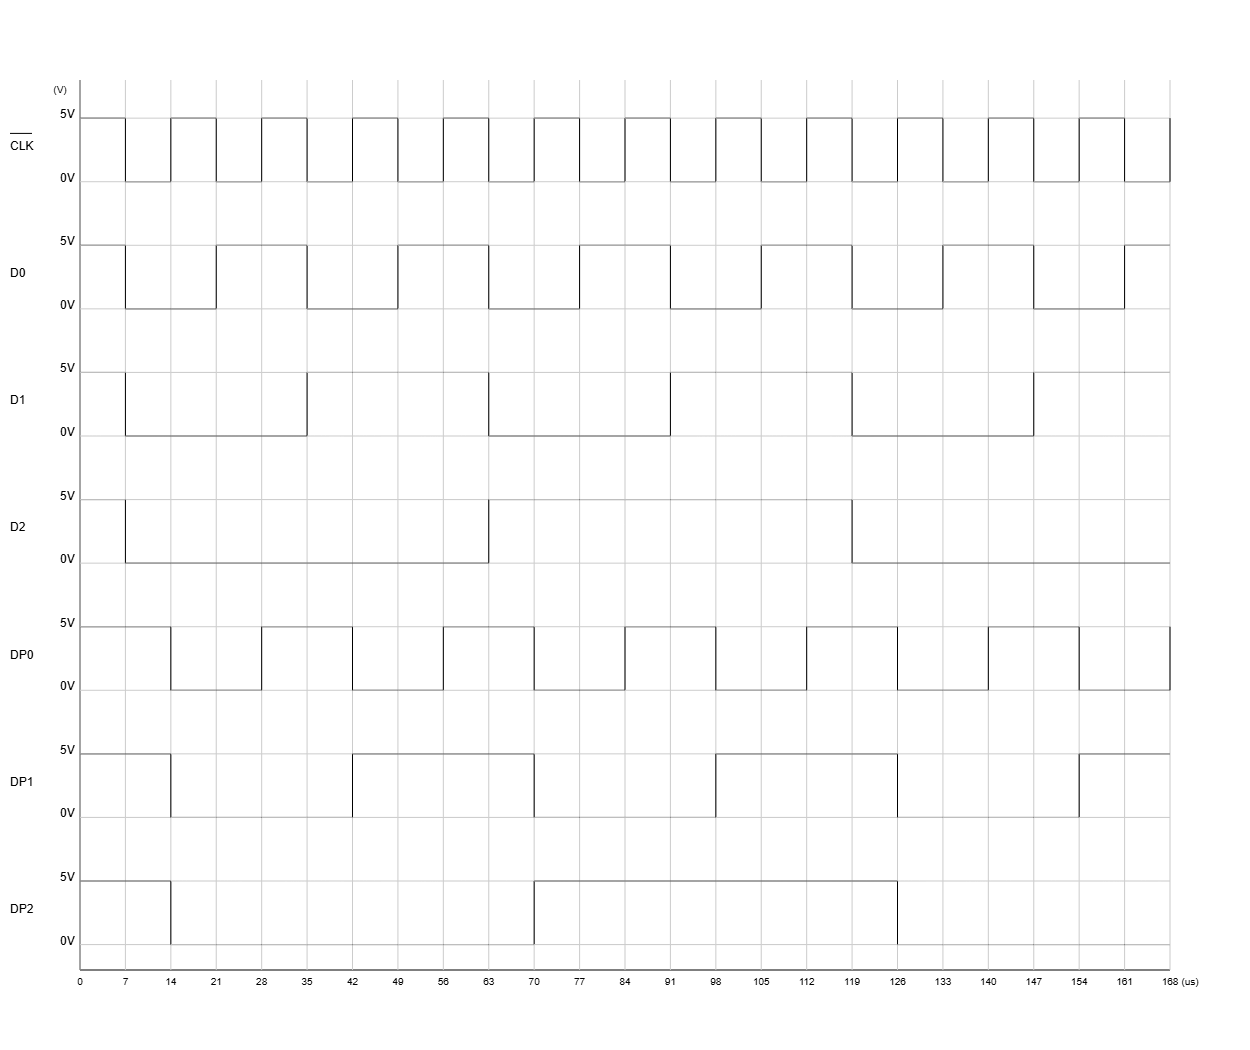
\includegraphics[width=1.0\linewidth]{./images/delay.png}
  \caption{遅延回路の波形}
  \label{fig:delay}
\end{figure}

\subsection{全体の動作確認}
全体の動作確認を行う.
デコーダ回路,セレクタ回路,減算回路をフラットケーブルに接続し,減算回路とA/D変換回路を接続する.
そして$AIN_0$を0[V]から5[V]まで変化させ,TP8の電圧の値が,0.04[V],0.68[V],1.20[V],1.80[V],2.40[V],3.00[V],3.50[V]になった時に
7セグメントLEDに0,1,2,3,4,5,6が表示されることを確認する.動作を表した表を表\ref{tab:operation}に示す。

\begin{table}[H]
  \centering
  \caption{全体の動作確認}
  \begin{tabular}{|c|c|c|c|c|c|c|c|c|c|}
    \hline
    $AIN_0$[V] & 0.64 & 1.48 & 2.08 & 2.52 & 3.28 & 3.52 & 4.92 \\
    \hline
    TP8[V] & 0.04 & 0.68 & 1.20 & 1.80 & 2.40 & 3.00 & 3.50 \\
    \hline
    7セグメントLEDの表示 & 1 & 2 & 3 & 4 & 5 & 6 & 7 \\
    \hline
  \end{tabular}
  \label{tab:operation}
\end{table}

\section{考察}
本実験では,A/D変換回路を利用し,アナログ信号とディジタル信号を比較することで,A/D変換の原理を理解することができた.
また,精度のいい回路を工作することによる正確な発振回路の設計や,デジタル信号をアナログ信号に変換するラダー回路の設計を行うことの重要さを学ぶことができた.


\section{参考文献}
\addcontentsline{toc}{section}{参考文献}
\begin{thebibliography}{99}
  \bibitem{densi}岩田 聡 著,『電子回路』,株式会社 オーム社,pp.99-107,2015年2月20日.
  \bibitem{digital}堀 桂太郎 著,『絵とき ディジタル回路入門早わかり』,株式会社 オーム社,pp.56-57 pp120-121,2016年7月13日.
\end{thebibliography}

\end{document}